\section{clipbrecords Class Reference}
\label{classclipbrecords}\index{clipbrecords@{clipbrecords}}
{\tt \#include $<$clipbrecords.h$>$}

Collaboration diagram for clipbrecords:\begin{figure}[H]
\begin{center}
\leavevmode
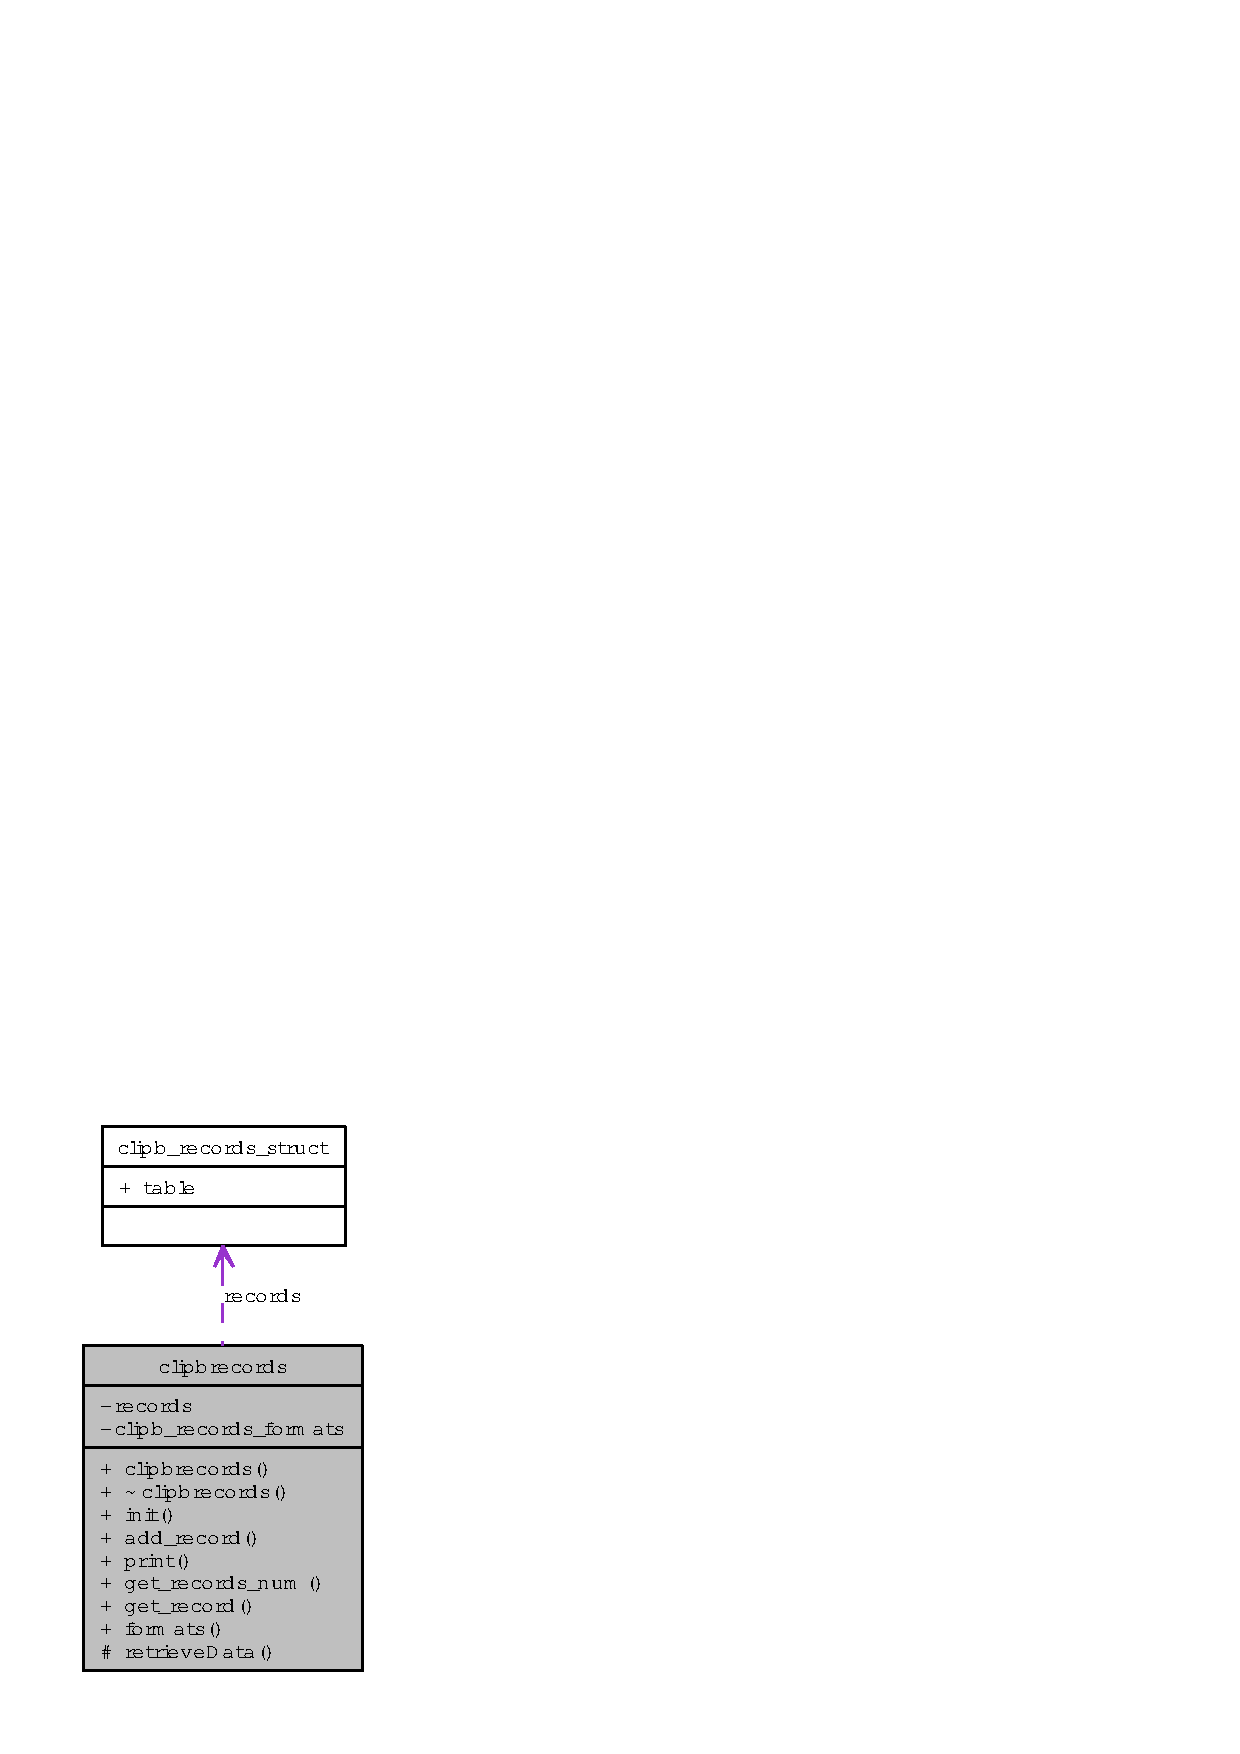
\includegraphics[width=89pt]{classclipbrecords__coll__graph}
\end{center}
\end{figure}
\subsection*{Public Member Functions}
\begin{CompactItemize}
\item 
{\bf clipbrecords} (void)
\item 
{\bf $\sim$clipbrecords} (void)
\item 
void {\bf init} (void)
\item 
void {\bf add\_\-record} (QMap$<$ QString, QString $>$ record)
\item 
void {\bf print} (void) const
\item 
int {\bf get\_\-records\_\-num} (void) const
\item 
QMap$<$ QString, QString $>$ {\bf get\_\-record} (int n) const
\item 
QString\-List {\bf formats} () const
\end{CompactItemize}
\subsection*{Protected Member Functions}
\begin{CompactItemize}
\item 
QVariant {\bf retrieve\-Data} (const QString \&format, QVariant::Type preferred\-Type) const
\end{CompactItemize}
\subsection*{Private Attributes}
\begin{CompactItemize}
\item 
{\bf clipb\_\-records\_\-struct} {\bf records}
\item 
QString\-List {\bf clipb\_\-records\_\-formats}
\end{CompactItemize}


\subsection{Detailed Description}




Definition at line 18 of file clipbrecords.h.

\subsection{Constructor \& Destructor Documentation}
\index{clipbrecords@{clipbrecords}!clipbrecords@{clipbrecords}}
\index{clipbrecords@{clipbrecords}!clipbrecords@{clipbrecords}}
\subsubsection{\setlength{\rightskip}{0pt plus 5cm}clipbrecords::clipbrecords (void)}\label{classclipbrecords_db47a32820dfe287ab51dac87d4cac8c}




Definition at line 11 of file clipbrecords.cpp.

References init().

Here is the call graph for this function:\begin{figure}[H]
\begin{center}
\leavevmode
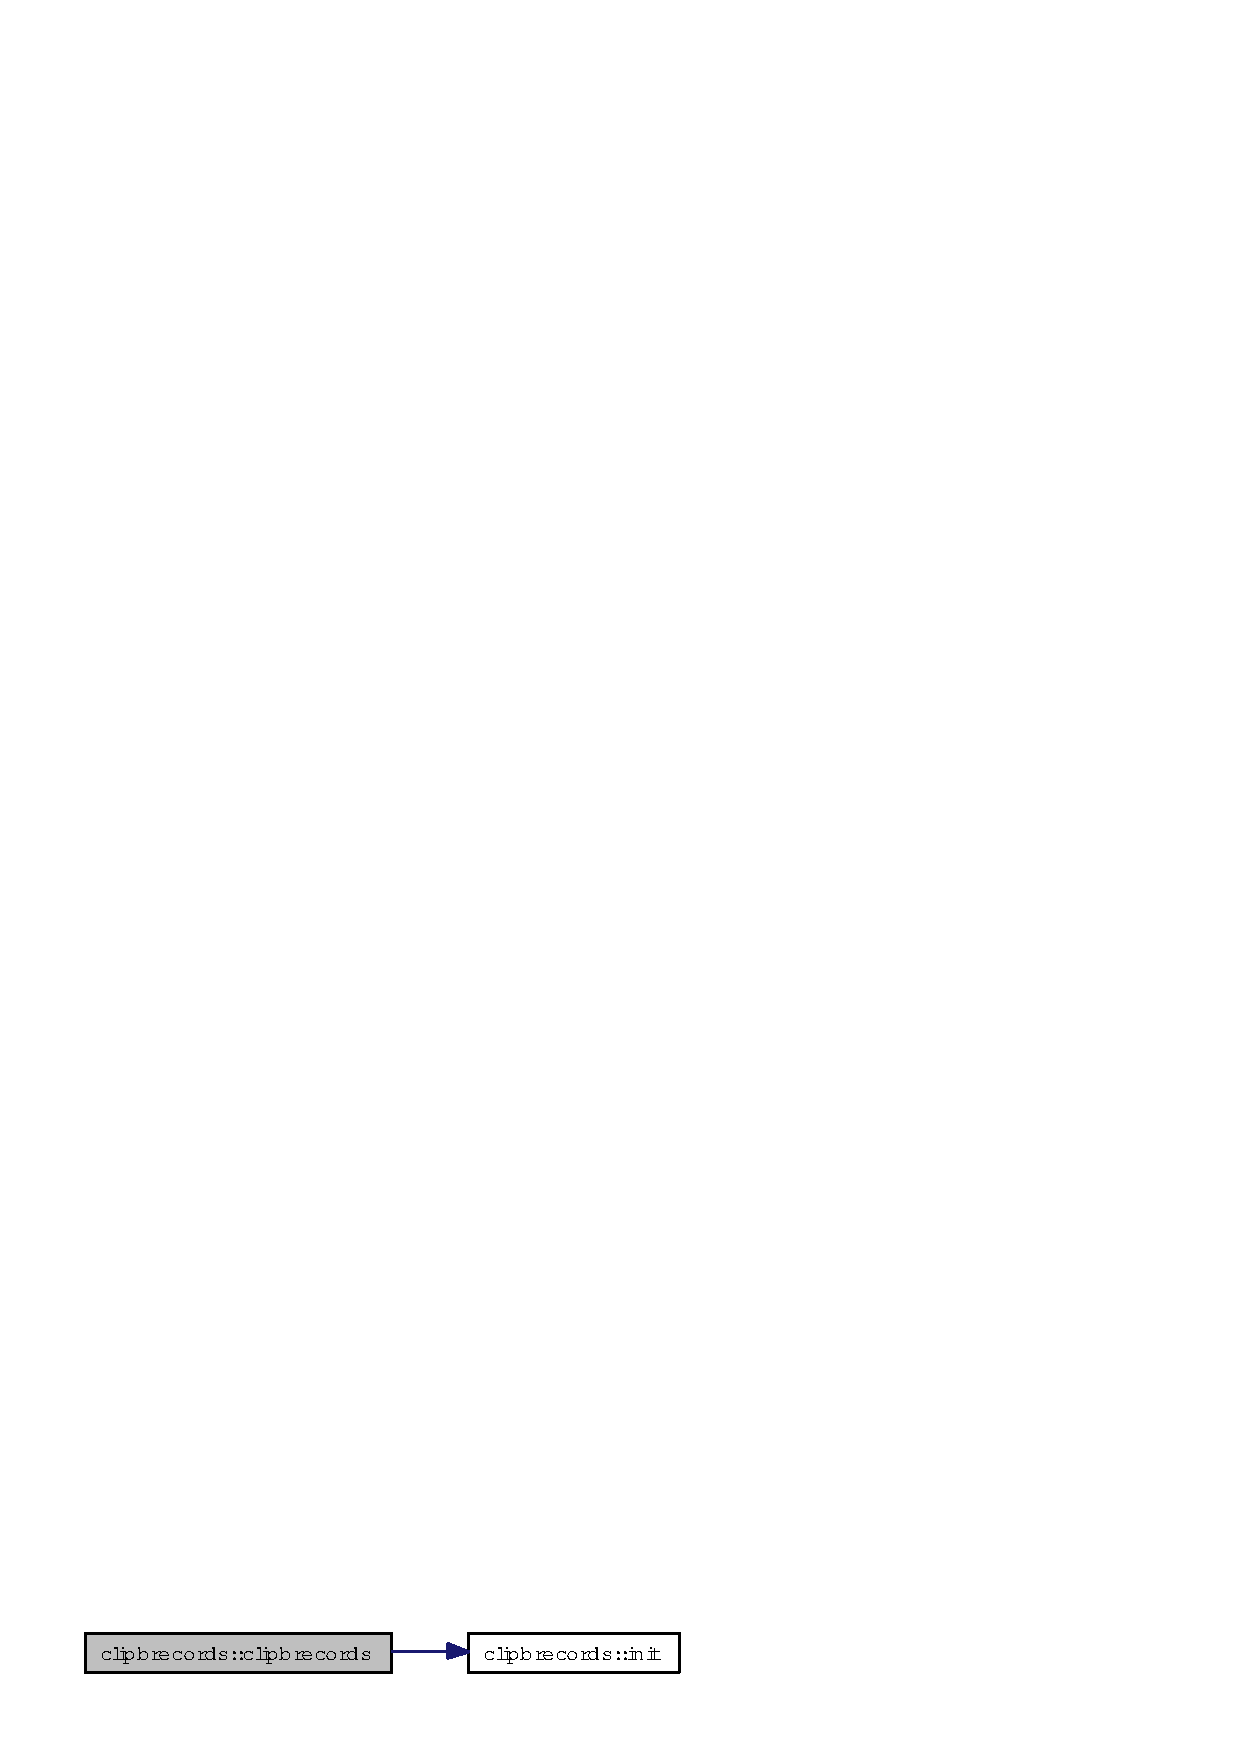
\includegraphics[width=165pt]{classclipbrecords_db47a32820dfe287ab51dac87d4cac8c_cgraph}
\end{center}
\end{figure}
\index{clipbrecords@{clipbrecords}!~clipbrecords@{$\sim$clipbrecords}}
\index{~clipbrecords@{$\sim$clipbrecords}!clipbrecords@{clipbrecords}}
\subsubsection{\setlength{\rightskip}{0pt plus 5cm}clipbrecords::$\sim$clipbrecords (void)}\label{classclipbrecords_8c498ef073b5796bd4a077d12c7c49e3}




Definition at line 17 of file clipbrecords.cpp.

\subsection{Member Function Documentation}
\index{clipbrecords@{clipbrecords}!init@{init}}
\index{init@{init}!clipbrecords@{clipbrecords}}
\subsubsection{\setlength{\rightskip}{0pt plus 5cm}void clipbrecords::init (void)}\label{classclipbrecords_8f9121a03c82d1d2ad32a81d19cbb1b7}




Definition at line 23 of file clipbrecords.cpp.

References clipb\_\-records\_\-formats, records, and clipb\_\-records\_\-struct::table.

Referenced by clipbrecords().

Here is the caller graph for this function:\begin{figure}[H]
\begin{center}
\leavevmode
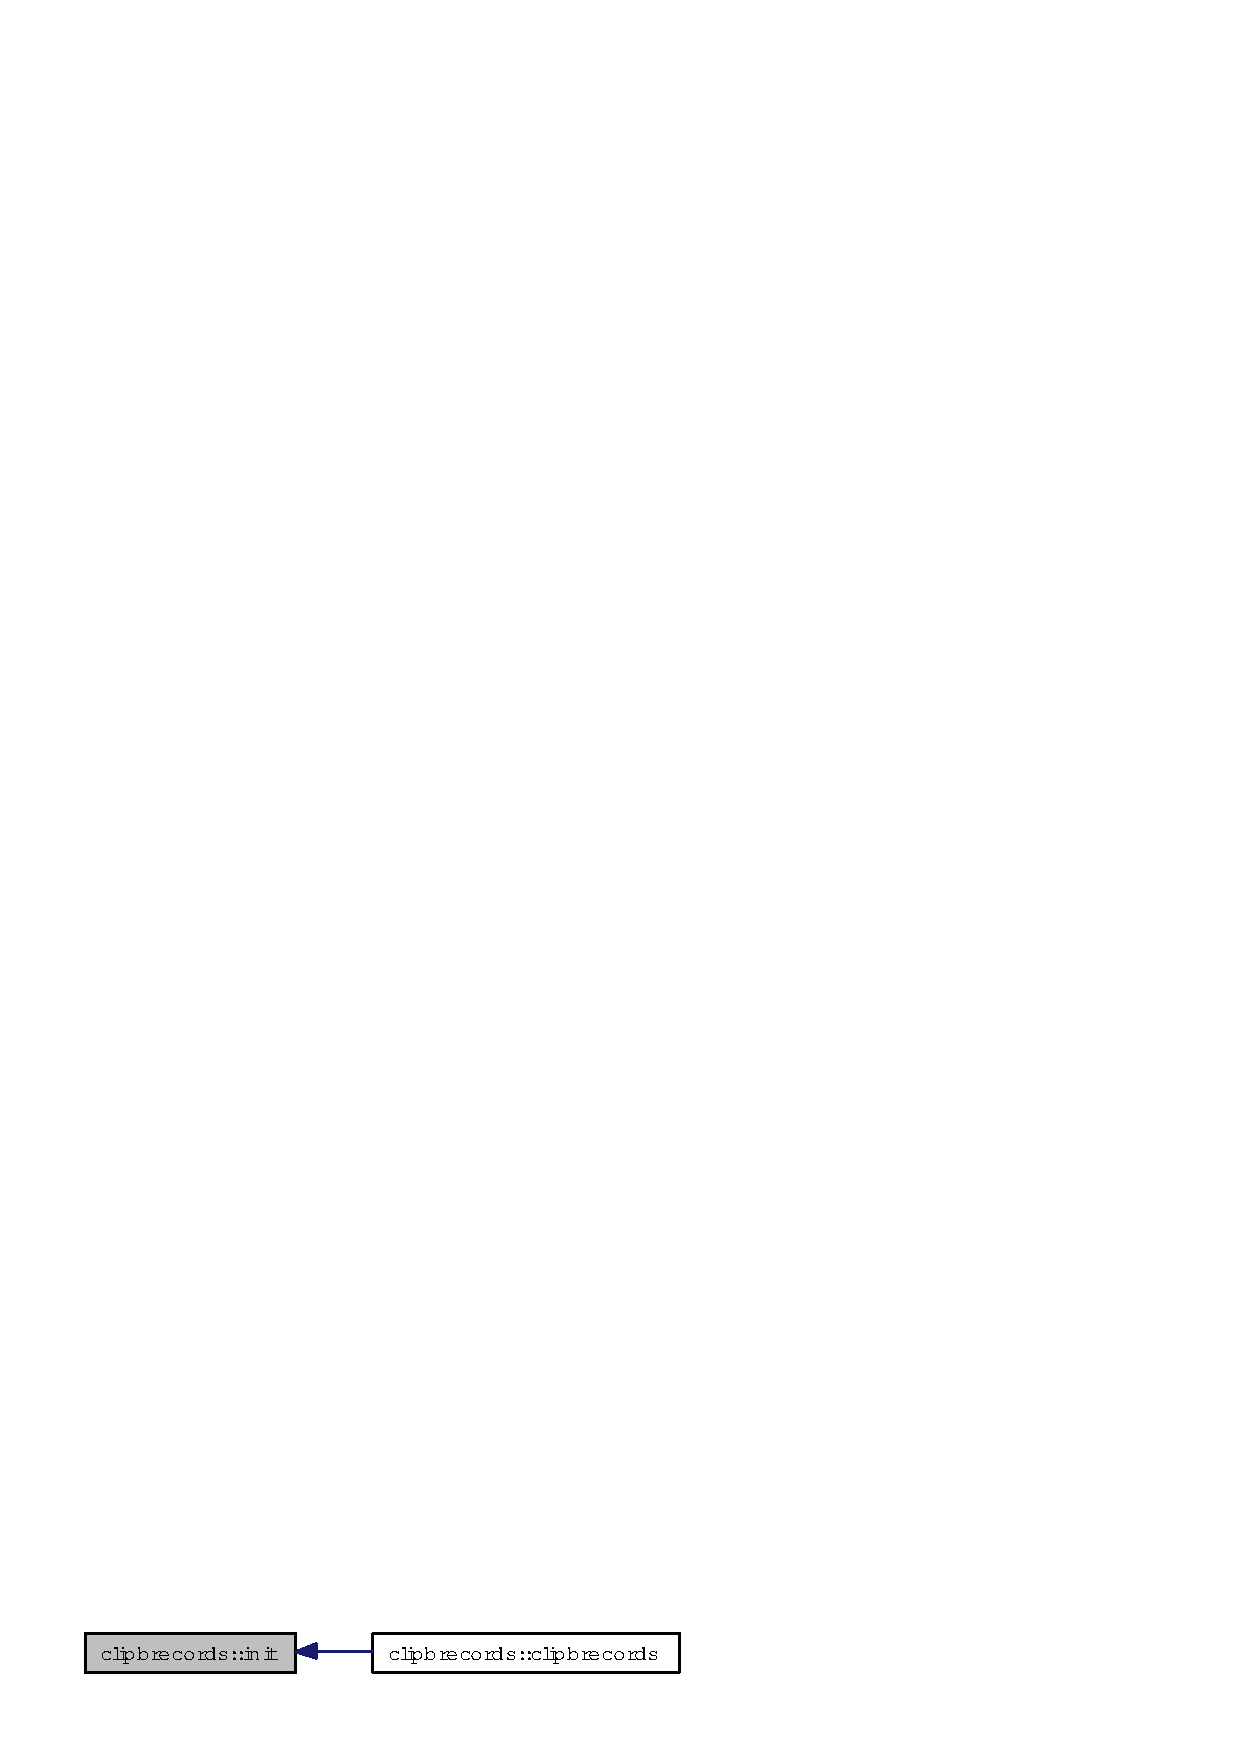
\includegraphics[width=165pt]{classclipbrecords_8f9121a03c82d1d2ad32a81d19cbb1b7_icgraph}
\end{center}
\end{figure}
\index{clipbrecords@{clipbrecords}!add_record@{add\_\-record}}
\index{add_record@{add\_\-record}!clipbrecords@{clipbrecords}}
\subsubsection{\setlength{\rightskip}{0pt plus 5cm}void clipbrecords::add\_\-record (QMap$<$ QString, QString $>$ {\em record})}\label{classclipbrecords_6321842c1409b39eaa0433b7e01845bb}




Definition at line 32 of file clipbrecords.cpp.

References records, and clipb\_\-records\_\-struct::table.

Referenced by recordtablescreen::copy().\index{clipbrecords@{clipbrecords}!print@{print}}
\index{print@{print}!clipbrecords@{clipbrecords}}
\subsubsection{\setlength{\rightskip}{0pt plus 5cm}void clipbrecords::print (void) const}\label{classclipbrecords_52fd489523b450d941fc81655bb80bdc}




Definition at line 38 of file clipbrecords.cpp.

References records, and clipb\_\-records\_\-struct::table.

Referenced by recordtablescreen::copy(), and recordtablescreen::paste().\index{clipbrecords@{clipbrecords}!get_records_num@{get\_\-records\_\-num}}
\index{get_records_num@{get\_\-records\_\-num}!clipbrecords@{clipbrecords}}
\subsubsection{\setlength{\rightskip}{0pt plus 5cm}int clipbrecords::get\_\-records\_\-num (void) const}\label{classclipbrecords_bb594290bb70e0dc9d66237ed272e173}




Definition at line 60 of file clipbrecords.cpp.

References records, and clipb\_\-records\_\-struct::table.

Referenced by recordtablescreen::paste().\index{clipbrecords@{clipbrecords}!get_record@{get\_\-record}}
\index{get_record@{get\_\-record}!clipbrecords@{clipbrecords}}
\subsubsection{\setlength{\rightskip}{0pt plus 5cm}QMap$<$ QString, QString $>$ clipbrecords::get\_\-record (int {\em n}) const}\label{classclipbrecords_539c2263d9314dc24cd47b833bbcac8a}




Definition at line 67 of file clipbrecords.cpp.

References critical\_\-error(), records, and clipb\_\-records\_\-struct::table.

Referenced by recordtablescreen::paste().

Here is the call graph for this function:\begin{figure}[H]
\begin{center}
\leavevmode
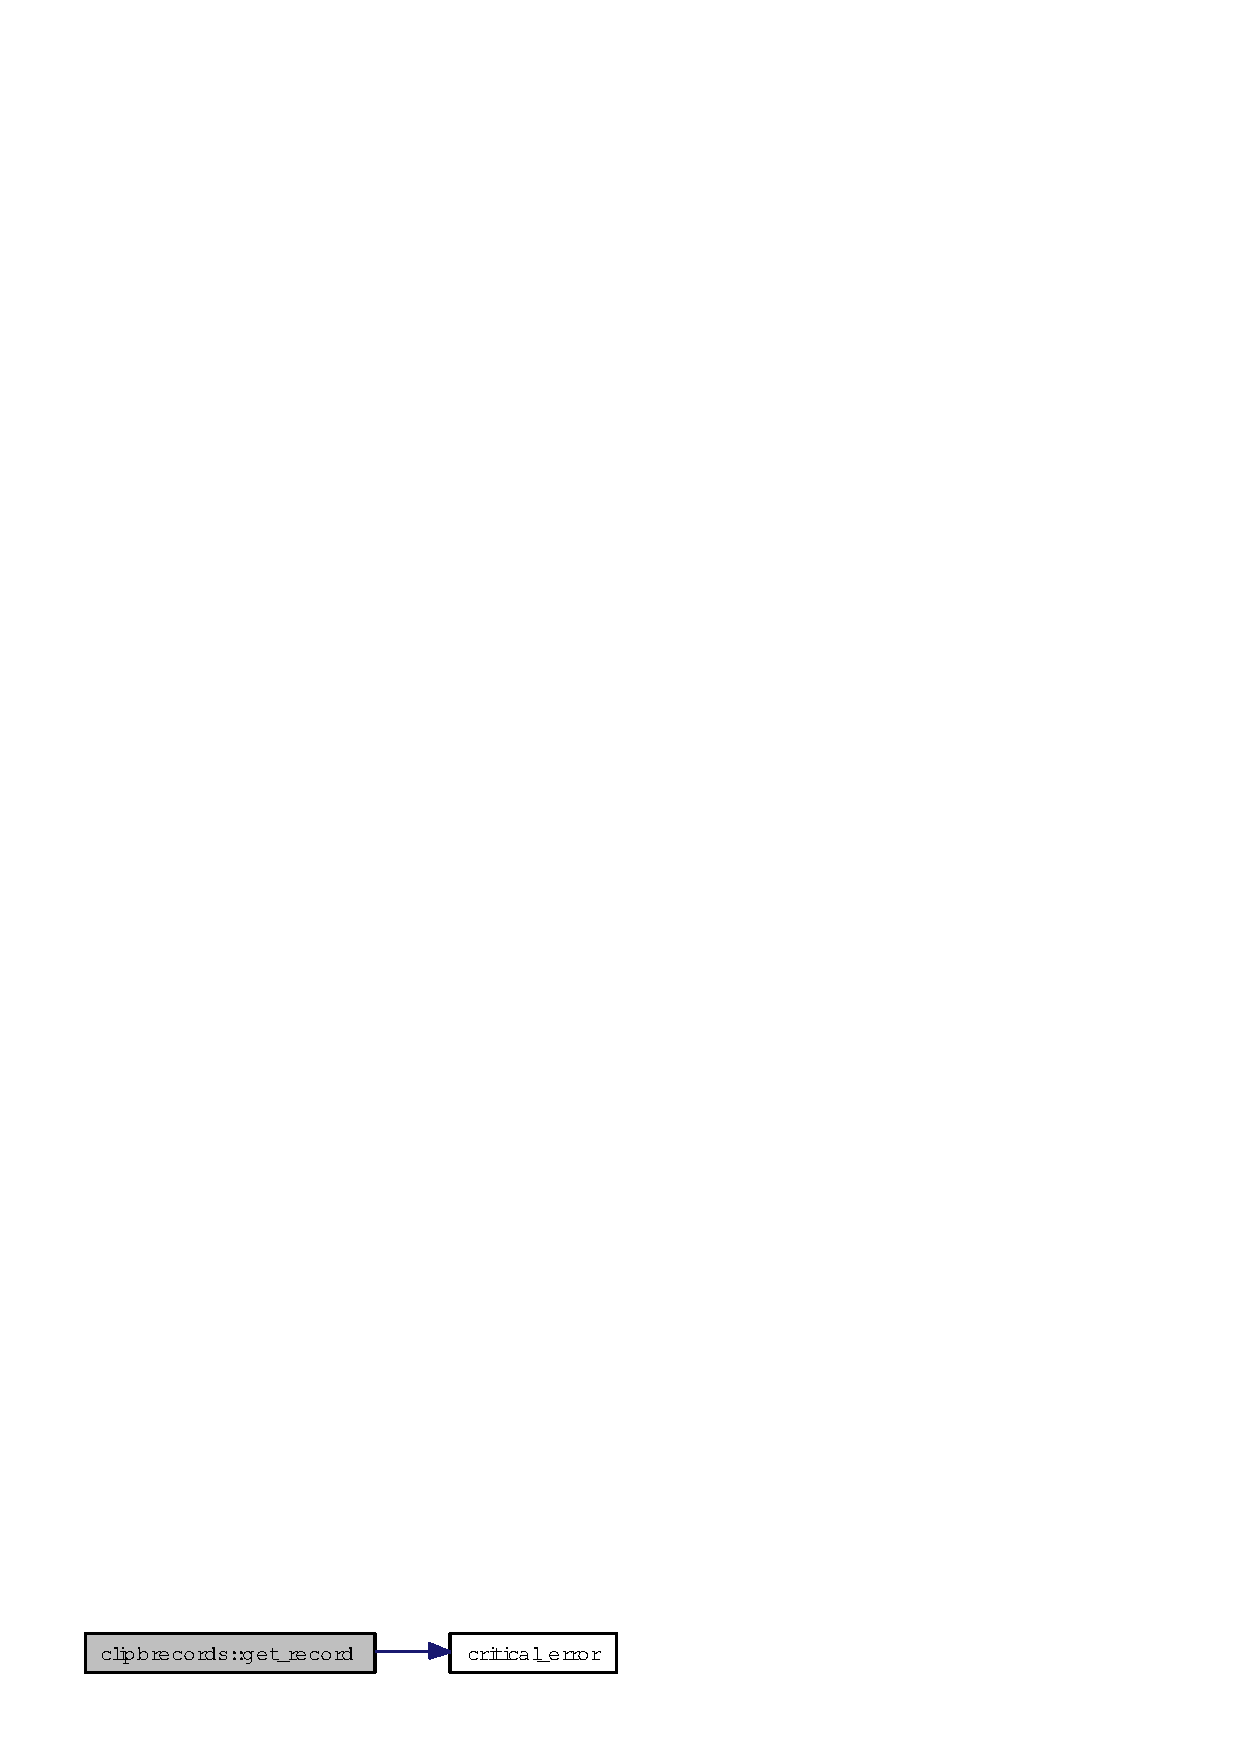
\includegraphics[width=150pt]{classclipbrecords_539c2263d9314dc24cd47b833bbcac8a_cgraph}
\end{center}
\end{figure}
\index{clipbrecords@{clipbrecords}!formats@{formats}}
\index{formats@{formats}!clipbrecords@{clipbrecords}}
\subsubsection{\setlength{\rightskip}{0pt plus 5cm}QString\-List clipbrecords::formats () const}\label{classclipbrecords_5cf9602a5d64022c46dd8a31479788a9}




Definition at line 79 of file clipbrecords.cpp.

References clipb\_\-records\_\-formats.\index{clipbrecords@{clipbrecords}!retrieveData@{retrieveData}}
\index{retrieveData@{retrieveData}!clipbrecords@{clipbrecords}}
\subsubsection{\setlength{\rightskip}{0pt plus 5cm}QVariant clipbrecords::retrieve\-Data (const QString \& {\em format}, QVariant::Type {\em preferred\-Type}) const\hspace{0.3cm}{\tt  [protected]}}\label{classclipbrecords_230af274633fd96ac5d144811d4798e5}




Definition at line 85 of file clipbrecords.cpp.

References records.

\subsection{Member Data Documentation}
\index{clipbrecords@{clipbrecords}!records@{records}}
\index{records@{records}!clipbrecords@{clipbrecords}}
\subsubsection{\setlength{\rightskip}{0pt plus 5cm}{\bf clipb\_\-records\_\-struct} {\bf clipbrecords::records}\hspace{0.3cm}{\tt  [private]}}\label{classclipbrecords_99b923d31bf749f7714e138b0d6bfc4b}




Definition at line 41 of file clipbrecords.h.

Referenced by add\_\-record(), get\_\-record(), get\_\-records\_\-num(), init(), print(), and retrieve\-Data().\index{clipbrecords@{clipbrecords}!clipb_records_formats@{clipb\_\-records\_\-formats}}
\index{clipb_records_formats@{clipb\_\-records\_\-formats}!clipbrecords@{clipbrecords}}
\subsubsection{\setlength{\rightskip}{0pt plus 5cm}QString\-List {\bf clipbrecords::clipb\_\-records\_\-formats}\hspace{0.3cm}{\tt  [private]}}\label{classclipbrecords_29f49b5fa69bd05e596a8909a03ab2d1}




Definition at line 42 of file clipbrecords.h.

Referenced by formats(), and init().

The documentation for this class was generated from the following files:\begin{CompactItemize}
\item 
{\bf clipbrecords.h}\item 
{\bf clipbrecords.cpp}\end{CompactItemize}
